\documentclass[final,t]{beamer}
\mode<presentation>
{
  \usetheme{MCSposter}
  \usecolortheme{default}
  \usefonttheme[onlymath]{serif}
}
\usepackage[orientation=landscape,size=custom,width=120,height=90,scale=1.3]{beamerposter}
%\usepackage[orientation=landscape,size=a0,scale=1.4]{beamerposter}
%\usepackage{pgfpages}
%\pgfpagesuselayout{resize to}[a4paper,landscape,border shrink=5mm]
%\pgfpagesuselayout{resize to}[a0paper,landscape]

% additional settings
\setbeamerfont{itemize}{size=\normalsize}
\setbeamerfont{itemize/enumerate body}{size=\normalsize}
\setbeamerfont{itemize/enumerate subbody}{size=\normalsize}

% additional packages
\usepackage{times}
\usepackage{subfig}
\usepackage{textpos}
\usepackage{wrapfig}
\usepackage{sidecap}
%\usepackage{sfmath} 
\usepackage{amsmath,amsthm,bm,microtype}
\usepackage{siunitx}
\DeclareSIUnit\year{a}
\sisetup{retain-unity-mantissa = false}
\usepackage{exscale}
\usepackage{multicol,multirow}
\usepackage{booktabs}
%\usepackage[english]{babel}
\usepackage[latin1]{inputenc}
\newcommand\todo[1]{{\color{red}\bf [TODO: #1]}}
\usepackage{tikz}
\usetikzlibrary{decorations.pathreplacing}
\usetikzlibrary{shadows,arrows,shapes.misc,shapes.arrows,shapes.multipart,arrows,decorations.pathmorphing,backgrounds,positioning,fit,petri,calc,shadows,chains,matrix}
\usepackage{fancyvrb}
\newcommand\cverb[1][]{\SaveVerb[%
    aftersave={\textnormal{\UseVerb[#1]{vsave}}}]{vsave}}

\bibliographystyle{unsrt-shortauthor}

%\def\newblock{\hskip .11em plus .33em minus .07em} % for natbib and beamer IMPORTANT
\listfiles
\graphicspath{{/home/jed/talks/figures/}{/home/jed/src/aterrel-presentations/figures/}}
% Display a grid to help align images
%\beamertemplategridbackground[1cm]

\newcommand\jedcolor[1]{{}}

\title{\huge On the utility of communication-avoiding and vectorization strategies in wave propagation analysis}
\author[Jed Brown]{Jed Brown {\texttt{jedbrown@mcs.anl.gov}}}
\institute[MCS]{Download this poster from \url{http://59A2.org/files/20130715-CIGQUEST.pdf}}

\newcommand{\newt}[1]{\tilde{#1}}
\newcommand{\btab}{\hspace{\stretch{1}}}
\newcommand{\C}{\mathbb{C}}
\newcommand{\N}{\mathbb{N}}
\newcommand{\Q}{\mathbb{Q}}
\newcommand{\R}{\mathbb{R}}
\newcommand{\Rz}{\mathcal{R}}
\newcommand{\RR}{{\bar{\mathbb{R}}}}
\newcommand{\II}{\mathcal{I}}
\newcommand{\Z}{\mathbb{Z}}
\newcommand{\Zp}{\mathbb{Z}_+}
\newcommand{\B}{\mathcal{B}}
\newcommand{\M}{\mathcal{M}}
\newcommand{\LL}{\mathcal{L}}
\newcommand{\PP}{\mathscr{P}}
\newcommand{\ff}{\bm f}
\newcommand{\uu}{\bm u}
\newcommand{\vv}{\bm v}
\newcommand{\ww}{\bm w}
\newcommand{\DD}{D}
\newcommand{\EE}{\mathcal E}
\newcommand{\VV}{\bm{\mathcal{V}}}
\newcommand{\Pspace}{\mathcal{P}}
\newcommand\pfrak{{\mathfrak p}}
\newcommand{\di}{\partial}
\newcommand{\bigO}{\mathcal{O}}
\newcommand{\abs}[1]{\left\lvert #1 \right\rvert}
\newcommand{\bigabs}[1]{\big\lvert #1 \big\rvert}
\newcommand{\norm}[1]{\left\lVert #1 \right\rVert}
\newcommand{\ceil}[1]{\left\lceil #1 \right\rceil}
\newcommand{\floor}[1]{\left\lfloor #1 \right\rfloor}
\newcommand{\dif}{\bigtriangleup}
\newcommand{\ud}{\,\mathrm{d}}
\newcommand{\tcolon}{\!:\!}
\DeclareMathOperator{\sgn}{sgn}
\DeclareMathOperator{\card}{card}
\DeclareMathOperator{\trace}{tr}
\DeclareMathOperator{\sspan}{span}
\renewcommand{\bar}{\overline}
\newcommand{\ed}{\dot{\epsilon}}

% abbreviations
\usepackage{xspace}
\makeatletter
\DeclareRobustCommand\onedot{\futurelet\@let@token\@onedot}
\def\@onedot{\ifx\@let@token.\else.\null\fi\xspace}
\def\eg{{e.g}\onedot} \def\Eg{{E.g}\onedot}
\def\ie{{i.e}\onedot} \def\Ie{{I.e}\onedot}
\def\cf{{c.f}\onedot} \def\Cf{{C.f}\onedot}
\def\etc{{etc}\onedot}
\def\vs{{vs}\onedot}
\def\wrt{w.r.t\onedot}
\def\dof{d.o.f\onedot}
\def\etal{{et al}\onedot}
\makeatother
%%%%%%%%%%%%%%%%%%%%%%%%%%%%%%%%%%%%%%%%%%%%%%%%%%%%%%%%%%%%%%%%%%%%%%%%%%%%%%%%%%%%%%%%%%%%%%%%%%%%%%%%%%%%

% Need to declare these here because newcommand inside a frame is fragile
\newcommand\mgdx{1.9em}
\newcommand\mgdy{2.5em}
\newcommand\mgloc[4]{(#1 + #4*\mgdx*#3,#2 + \mgdy*#3)}
\newcommand{\mglevel}{\ensuremath{\ell}}
\newcommand{\mglevelcp}{\ensuremath{\mglevel_{\mathrm{cp}}}}
\newcommand{\mglevelfine}{\ensuremath{\mglevel_{\mathrm{fine}}}}

\begin{document}
\begin{frame}{} 
  \vspace{-3em}
  \begin{columns}
    \begin{column}{0.31\textwidth}
      \begin{block}{Demand for strong scalability}
        The possibility of using inversion as a design or decision-making tool places markedly increased emphasis on turn-around time.
        While multi-day simulation turn-around may be acceptable for high-latency decisions, it is not sufficient for informing low-latency decisions such as arise in preliminary field surveys.
        The ability to use increased parallelism to reduce turn-around time for a fixed model resolution is known as ``strong scalability''.
        Strong scalability always saturates at some point, beyond which more cores provide no further benefit.
        With good implementation and hardware, the cost per iteration at the strong scaling limit is independent of global problem size.

      % Scaling time-accurate wave propagation
        Given a constant acceptable turn-around time, increasing resolution \emph{decreases} the time available per iteration.
        For example, isotropic refinement of a 3D model increases the number of grid points by $2^3 = 8$ as well as increasing the number of time steps by 2.
        With ideal scaling, we use 16 times as many cores so that the subdomain sizes is halved and we can complete steps in half the time.
        This quickly lands us in a latency-sensitive strong scaling regime.
      \end{block}

      % \begin{block}{Communication costs, memory locality, and vectorization}
      %   Efficient utilization of modern hardware is requiring increasingly fine-grained parallelism, latency-tolerance, memory locality for deep NUMA hierarchies, and various forms of vectorization.
      %   These approaches have varying costs and benefits, as well as far-reaching consequences on programming tools, software design, and the suitability of emerging hardware architectures.
      % \end{block}
      \vspace{-2em}

      \begin{block}{Communication amortization: $s$-step methods}
        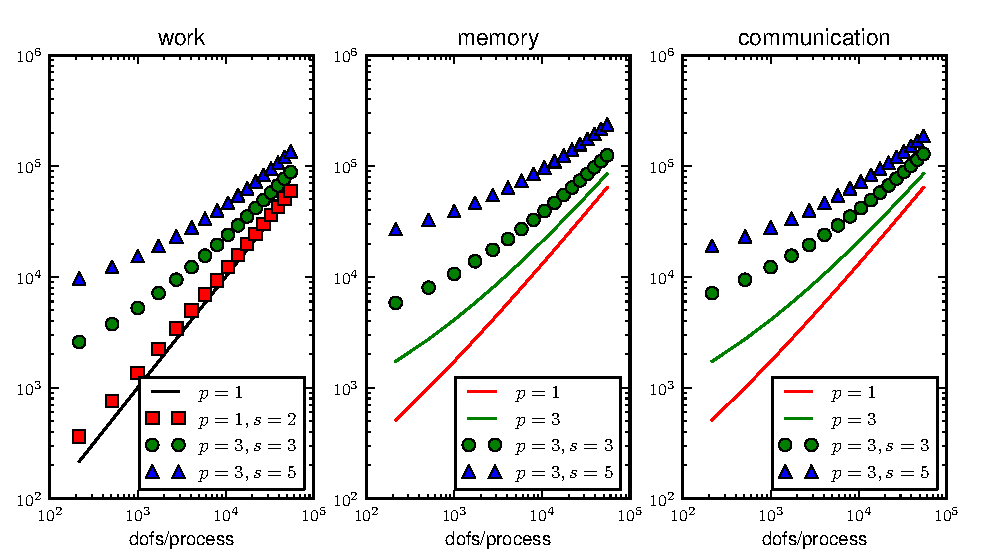
\includegraphics[width=1\textwidth]{figures/SStepEfficiencyP3.pdf}
        \begin{itemize}
        \item Amortizing message latency is most important for strong-scaling
        \item $s$-step methods have high overhead for small subdomains
        \item $s$-step overhead grows rapidly for high-order spatial discretization (especially spectral element)
        \item Aggregation and vectorization in stochastic dimension avoids this overhead, opportunity for reuse and mixing
        \end{itemize}
      \end{block}
      \vspace{-2em}
      \begin{block}{Can accelerators accelerate simulation turn-around?}
        \begin{itemize}
        \item MPI messaging latency: 1--10 microseconds
        \item GPU kernel launch overhead: about 20 microseconds
        \item \texttt{MPI\_Allreduce}: 20 microseconds on $10^6$ cores
        \item At least two kernel launches needed for non-overlapping writes (otherwise almost every write needs to be atomic)
        \item GPU trend: more threads, fewer registers, less shared memory
        \end{itemize}
      \end{block}

      % \begin{block}{Matrix-free for performance}
      %   \begin{wrapfigure}{r}{0.6\textwidth}
      %     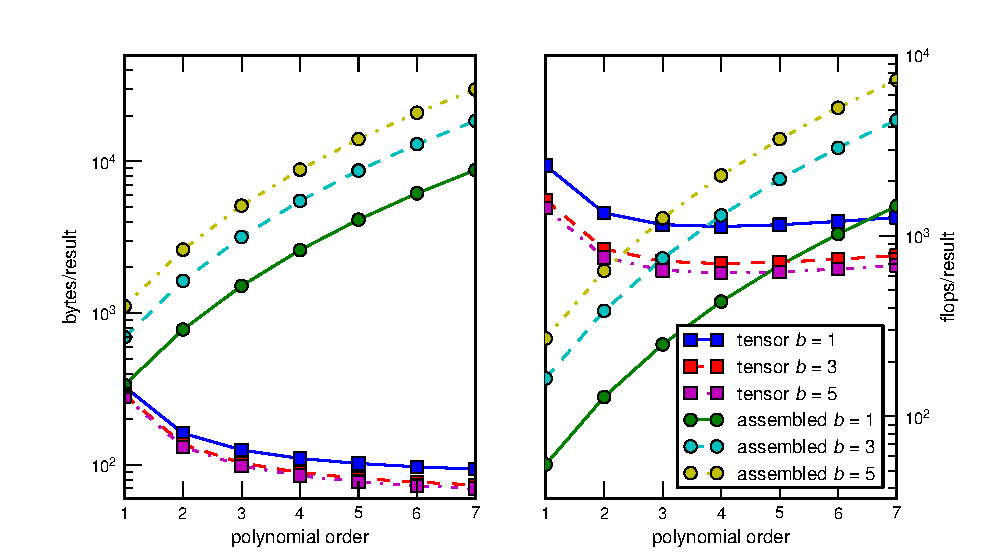
\includegraphics[width=0.58\textwidth]{figures/TensorVsAssembly}
      %     \caption{Relative cost in memory bandwidth and flops to apply
      %       linearized PDE operator arising in $p$-version finite
      %       element discretization of nonlinear PDEs with $b=1,3,5$
      %       degrees of freedom per node.}\label{fig:TensorVsAssembly}
      %   \end{wrapfigure}
      %   Assembled sparse matrices have long been a preferred representation for PDE operators, but are a remarkably poor fit for modern hardware due to memory bandwidth requirements.
      %   A matrix-vector product computed using an assembled matrix cannot have an arithmetic intensity higher than $1/4$, leaving modern floating point hardware severely under-utilized.
      %   \begin{table}
      %     \centering
      %     \begin{tabular}{lrrr}
      %       \toprule
      %       Processor           & BW (GB/s) & Peak (GF/s) & Balanced AI (F/B) \\
      %       \midrule
      %       Sandy Bridge 6-core & 21*       & 150         & 7.2                 \\
      %       Magny Cours 16-core & 42*       & 281         & 6.7                 \\
      %       Blue Gene/Q node    & 43        & 205         & 4.8                 \\
      %       % GeForce 9400M       & 21        & 54          & 2.6                 \\
      %       % GTX 285             & 159       & 1062        & 6.8                 \\
      %       Tesla M2090         & 120  & 665  & 5.5 \\
      %       Kepler K20Xm        & 160 & 1310 & 8.2 \\ % http://www.elekslabs.com/2012/11/nvidia-tesla-k20-benchmark-facts.html
      %       \bottomrule
      %     \end{tabular}
      %     \caption{Balanced arithmetic intensity (flops/byte) for several architectures.}\label{tab:BalancedAI}
      %   \end{table}
      % \end{block}
    \end{column}
    %
    \begin{column}{0.31\textwidth}
      \begin{block}{Parallel-in-time integrators}
        Parareal, parallel spectral deferred correction (SDC), and related methods have received attention recently for their strong scaling potential.
        Closely related (though neglected by much of the post-2000 literature, but see \cite{gander2007analysis}) is the space-time multigrid analysis from the 1980s and 1990s~\cite{vandewalle1995fourier,horton1995polylog,brandt1991parabolic}.
        Parareal and PFASST are Full Approximation Scheme (FAS) multigrid algorithms with spatially coupled smoothers.
        The equivalent of SDC has a long history in multigrid: high-order discretizations have poor $h$-ellipticity which makes them unsuitable for smoothers except as a residual evaluation to be corrected using an $h$-elliptic discretization.
        Common attributes of the current generation of parallel-in-time integrators:
        \begin{itemize}
        \item Efficiency is always low.  For stability-limited integration, the efficiency of PFASST~\cite{emmett2012toward} and related algorithms on $N$ processors is bounded by
          \begin{equation*}
            E < \frac{1}{N \alpha + K_p (1 + \alpha + \beta)}
          \end{equation*}
          where $K_p$ is the number of iterations to converge, $\alpha$ is the time spent in the coarse integrator on each iteration in units of (parallel) fine-grid corrections, and $\beta$ is the communication cost.
        \item Conventional coarse grids cannot represent high frequencies accurately, but high-frequency \emph{waves} cannot be resolved \emph{locally} on fine grid.
        \item New homogenization results needed to avoid $K_p \sim N$~\cite{gander2008hyperbolic} for waves.
        \item For hyperbolic problems with multiple wave speeds, the essential coupling rank is higher in the time dimension than in spatial dimensions.
        \item Waveform relaxation: much higher efficiency for parabolic problems, but only constant factor improvement for hyperbolic (ratio of wave speeds).
        \item Implies chunky space-time subdomains, likely ``longer'' in time direction.
        \end{itemize}
      \end{block}
      \vspace{-2em}
      \begin{block}{A notion of coupling rank}
        \begin{itemize}
        \item ``Full space'' (spatial, temporal, parameters, stochastic, \ldots)
        \end{itemize}
        \vspace{-1em}
        \begin{figure}
          \centering
          \begin{tikzpicture}
            [>=stealth,
            scale=2,every node/.style={scale=1,font=\scriptsize}
            ]
            \draw (0,0) circle [x radius=1.6, y radius=1, rotate=-20] node[below] {input space};
            \draw (4,0) circle [x radius=1.6, y radius=1, rotate=20] node[below] {output space};
            % \draw (0.5,0.5) circle [radius=.3] node{$U$};
            % \draw (3.6,0.6) circle [x radius=.2, y radius=.3] node{$V$};
            \node[circle,radius=.3,draw] (U) at (0.5,0.3) {$U$};
            \node[circle,x radius=.2,y radius=.3,draw] (V) at (3.5,0.3) {$V$};
            \draw[->] (U) to[out=20,in=150] node[above] {$A_{V,U}$} (V);
          \end{tikzpicture}
        \end{figure}
        \vspace{-1em}
        \begin{itemize}
        \item $A_{V,U}$: dependence of solution in subdomain $V$ on data from subdomain $U$
        \item Essential rank $k$ of $A_{V,U}$: number of singular values $>$ relative tolerance
        \item Crude lower bound: at least $k$ units of information must be communicated from $U$ to $V$
        \item Parallel distribution: high-rank couplings should be ``nearby''
        \end{itemize}
        \begin{figure}
          \centering
          \begin{tikzpicture}[ scale=2,every
            node/.style={scale=1,font=\scriptsize}, >=stealth,
            uset/.style={draw=blue!40!black,fill=blue!10,rounded
              corners},
            vset/.style={draw=red!40!black,fill=red!10,rounded corners}
            ]
            \draw (0,0) grid[xstep=0.1,ystep=3] (3,3); \draw (4,0)
            grid[xstep=0.1,ystep=3] (7,3); \node[uset,minimum width=3cm]
            (Uunaligned) at (1.5,2.5) {$U$}; \node[vset,minimum
            width=3cm] (Vunaligned) at (1.5,0.5) {$V$};
            \node[uset,minimum height=3cm] (Ualigned) at (4.5,1.5)
            {$U$}; \node[vset,minimum height=3cm] (Valigned) at
            (6.5,1.5) {$V$}; \draw[->,thick] (Uunaligned) --
            node[fill=gray!10] {High-rank} (Vunaligned); \draw[->,thick]
            (Ualigned) -- node[fill=green!10,above] {Weak} (Valigned);
          \end{tikzpicture}
        \end{figure}
        \begin{itemize}
        \item Identical distribution for input and output spaces is natural.
        \item The $k$ items of data can be communicated in different ways:
          \begin{itemize}
          \item Increasingly-large subdomains at greater distance (tree-code)
          \item Interaction through coarse grid (multigrid, fast multipole)
          \end{itemize}
        \end{itemize}
      \end{block}

    \end{column}
    %
    \begin{column}{0.31\textwidth}
      \begin{block}{The $\tau$ formulation of FAS multigrid}
        If hardware becomes much less reliable (predicted by some, not by others), inexpensive checkpointing and recovery will be needed.
        Writing to globally-visible memory is rapidly becoming untenable, currently taking about an hour to read or write the contents of memory.
        We outline a multiscale compressed checkpointing scheme based on Full Approximation Scheme (FAS) multigrid used either as an accelerator to quasi-Newton optimization methods or in space-time.
        \begin{itemize}
        \item classical formulation: ``coarse grid \emph{accelerates} fine grid solution''
        \item $\tau$ formulation: ``fine grid improves accuracy of coarse grid''
        \item To solve $N u = f$, recursively apply
          \begin{equation*}
            \begin{split}
              \text{pre-smooth} \:\: & \quad \tilde u^h \gets S^h_{\text{pre}}(u^h_0, f^h) \\
              \text{solve coarse problem for $u^H$} \:\: & \quad N^H u^H = \underbrace{I_h^H f^h}_{f^H} + \underbrace{N^H \hat I_h^H \tilde u^h - I_h^H N^h \tilde u^h}_{\tau_h^H} \\
              \text{correction and post-smooth} \:\: & \quad u^h \gets S^h_{\text{post}} \Big( \tilde u^h + I_H^h (u^H - \hat I_h^H \tilde u^h), f^h \Big) \\
            \end{split}
          \end{equation*}
          \begin{tabular}{llll}
            \toprule
            $I_h^H$ & residual restriction & $\hat I_h^H$ & solution restriction \\
            $I_H^h$ & solution interpolation & $f^H = I_h^H f^h$ & restricted forcing \\
            $\{S^h_{\text{pre}},S^h_{\text{post}}\}$ & \multicolumn{3}{l}{smoothing operations on the fine grid} \\
            \bottomrule
          \end{tabular}
        \item At convergence, $u^{H*} = \hat I_h^H u^{h*}$ solves the $\tau$-corrected coarse grid equation
            $N^H u^H = f^H + \tau_h^H$,
          thus $\tau_h^H$ is the ``fine grid feedback'' that makes the coarse grid equation accurate.
        \end{itemize}
      \end{block}

      \vspace{-2em}
      \begin{block}{Multiscale compression and decompression}
        \begin{tikzpicture}
          [scale=0.7,every node/.style={scale=0.7},
          >=stealth,
          restrict/.style={thick,double},
          prolong/.style={thick,double},
          cprestrict/.style={green!50!black,thick,double,dashed},
          control/.style={rectangle,red!40!black,draw=red!40!black,thick},
          mglevel/.style={rounded rectangle,draw=blue!50!black,fill=blue!20,thick,minimum size=6mm},
          checkpoint/.style={rectangle,draw=green!50!black,fill=green!20,thick,minimum size=6mm},
          mglevelhide/.style={rounded rectangle,draw=gray!50!black,fill=gray!20,thick,minimum size=6mm},
          tau/.style={text=red!50!black,draw=red!50!black,fill=red!10,inner sep=1pt},
          crelax/.style={text=green!50!black,fill=green!10,inner sep=0pt}
          ]
          \begin{scope}
            \node[mglevel] (fine0) at \mgloc{0}{0}{4}{-1} {\mglevelfine};
            \node[mglevel] (finem1down0) at \mgloc{0}{0}{3}{-1} {};
            \node[mglevel] (cp1down0) at \mgloc{0}{0}{2}{-1} {$\mglevelcp+1$};
            \node[mglevel] (cpdown0) at \mgloc{0}{0}{1}{-1} {\mglevelcp};
            \node[mglevel] (coarser0) at \mgloc{0}{0}{0}{0} {\ldots};

            \node[mglevelhide] (cpup0) at \mgloc{0}{0}{1}{1} {};
            \node (cp1up0) at \mgloc{0}{0}{2}{1} {};

            \node (cpdown1) at \mgloc{4em}{0}{1}{-1} {};
            \node[mglevelhide] (coarser1) at \mgloc{4em}{0}{0}{1} {\ldots};
            \node[mglevel] (cpup1) at \mgloc{4em}{0}{1}{1} {\mglevelcp};
            \node[mglevel] (cp1up1) at \mgloc{4em}{0}{2}{1} {$\mglevelcp+1$};
            \node[mglevel] (finem1up1) at \mgloc{4em}{0}{3}{1} {};
            \node[mglevel] (fine1) at \mgloc{4em}{0}{4}{1} {\mglevelfine};

            \draw[->,restrict,dashed] (fine0) -- (finem1down0);
            \draw[->,restrict] (finem1down0) -- (cp1down0);
            \draw[->,restrict] (cp1down0) -- (cpdown0);
            \draw[->,restrict,dashed] (cpdown0) -- (coarser0);
            \draw[->,prolong,dashed] (coarser0) -- (cpup0);
            \draw[->,prolong,dashed] (cpup0) -- (cp1up0);

            \draw[->,restrict,dashed] (cpdown1) -- (coarser1);
            \draw[->,prolong,dashed] (coarser1) -- (cpup1);
            \draw[->,prolong] (cpup1) -- (cp1up1);
            \draw[->,prolong] (cp1up1) -- (finem1up1);
            \draw[->,prolong,dashed] (finem1up1) -- (fine1);

            \node[checkpoint] at (4em + \mgdx*4,\mgdy) (cp) {CP};
            \draw[>->,cprestrict] (fine1) -- node[below,sloped] {Restrict} (cp);

            \node[left=\mgdx of fine0] (bnanchor) {};
            \node[control,fill=red!20] at (1.1*\mgdx,3*\mgdy) {Solve $F(u^n;b^n) = 0$};
            \node[mglevel,right=of fine1] (finedt) {next solve};
            \draw[->, >=stealth, control] (fine1) to[out=20,in=170] node[above] {$b^{n+1}(u^n,b^n)$} (finedt);
            \draw[->, >=stealth, control] (bnanchor) to[out=45,in=155] node[above] {$b^n$} (fine0);

            % Recovery process
            \begin{scope}[xshift=8*\mgdx]
              \node[checkpoint] (rcp) at \mgloc{0}{0}{0}{0} {CP};
              \node[mglevel] (r0a) at \mgloc{0}{\mgdy}{0}{0} {CR};
              \node[mglevel] (r1a) at \mgloc{0}{\mgdy}{1}{1} {};
              \node[mglevel] (r0b) at \mgloc{2*\mgdx}{\mgdy}{0}{0} {CR};
              \node[mglevel] (r1b) at \mgloc{2*\mgdx}{\mgdy}{1}{1} {};
              \node[mglevel] (r2b) at \mgloc{2*\mgdx}{\mgdy}{2}{1} {\mglevelfine};
              \node[mglevel] (r1c) at \mgloc{6*\mgdx}{\mgdy}{1}{-1} {};
              \node[mglevel] (r0d) at \mgloc{6*\mgdx}{\mgdy}{0}{0} {CR};
              \node[mglevel] (r1d) at \mgloc{6*\mgdx}{\mgdy}{1}{1} {};
              \node[mglevel] (r2d) at \mgloc{6*\mgdx}{\mgdy}{2}{1} {\mglevelfine};

              \draw[-,prolong,green!50!black] (rcp) -- (r0a);
              \draw[->,prolong] (r0a) -- (r1a);
              \draw[->,restrict] (r1a) -- (r0b);
              \draw[->,restrict] (r0b) -- (r1b);
              \draw[->,restrict,dashed] (r1b) -- (r2b);
              \draw[->,restrict,dashed] (r2b) -- (r1c);
              \draw[->,restrict] (r1c) -- (r0d);
              \draw[->,restrict] (r0d) -- (r1d);
              \draw[->,restrict,dashed] (r1d) -- (r2d);

              \foreach \smooth in {finem1down0, cp1down0, cpdown0, coarser0,
                cpup1, cp1up1, finem1up1,
                r0b,r1c,r0d,r1d} {
                \node[above left=-5pt of \smooth.west,tau] {$\tau$};
              }
              \node[rectangle,fill=none,draw=green!50!black,thick,fit=(rcp)(r2d)] (recoverbox) {};
              \node[rectangle,draw=green!50!black,fill=green!20,thick,minimum size=6mm,above={0cm of recoverbox.south east},anchor=south east] (recover) {FMG Decompression};
            \end{scope}
            \node (notation) at (2*\mgdx,5*\mgdy) {
              \begin{minipage}{18em}\small\sf
                \begin{itemize}\addtolength{\itemsep}{-5pt}
                \item checkpoint converged coarse state
                \item recover using FMG anchored at $\mglevelcp+1$
                \item needs only $\mglevelcp$ neighbor points
                \item $\tau$ correction is local
                \end{itemize}
              \end{minipage}
            };
          \end{scope}
        \end{tikzpicture}
        \begin{itemize}
        \item Fine state $u^{h*}$ recovered \emph{locally} from converged coarse state $u^{H*} = \hat I_h^H u^{h*}$
        \item Normal multigrid cycles visit all levels moving from $n \to n+1$
        \item FMG recovery only accesses levels finer than $\ell_{CP}$
        \item Postprocessing applications, e.g., in-situ visualization at high temporal resolution in part of the domain
        \end{itemize}
      \end{block}      

      % \begin{block}{Local decompression and resilience}
      %   \begin{tikzpicture}
      %     [scale=1,every node/.style={scale=1},
      %     >=stealth,
      %     control/.style={rectangle,rounded corners,draw=blue!50!black,fill=blue!20,thick,minimum width=5em},
      %     essential/.style={rectangle,rounded corners,draw=red!50!black,fill=red!20,thick,minimum width=5em},
      %     ephemeral/.style={rectangle,rounded corners,draw=gray!50!black,fill=gray!20,thick,minimum width=5em},
      %     statebox/.style={rectangle,draw=green!50!black,thick},
      %     statetitle/.style={rectangle,draw=green!50!black,fill=green!20,thick},
      %     storebox/.style={rectangle,draw=},
      %     rightbrace/.style={decorate,decoration={brace,amplitude=1ex,raise=4pt}},
      %     leftbrace/.style={decorate,decoration={brace,amplitude=1ex,raise=4pt,mirror}}
      %     ]
      %     \scriptsize
      %     \node[control,minimum width=8em] (progcontrol) {control};
      %     \node[essential,below=2pt of progcontrol.south,rectangle split,rectangle split parts=2,rectangle split horizontal,minimum width=12em] (progessential) {essential \nodepart{two} coarse};
      %     \node[ephemeral,minimum width=8em,below=2pt of progessential.south] (progephemeral) {ephemeral};
      %     \node[statebox,fit=(progcontrol)(progessential)(progephemeral)] (progbox) {};
      %     \node[above=0pt of progbox.north,anchor=south] {\textbf{program $n=0$}};

      %     \node[control,right=9em of progcontrol] (storecontrol) {control};
      %     \node[essential,below=2pt of storecontrol.south] (storeessential) {essential};
      %     \node[essential,minimum width=4em,below=6pt of storeessential.south, double copy shadow] (storecoarse) {coarse};
      %     \node[statebox,decorate,decoration={bumps,mirror},fit=(storecontrol)(storecoarse)] (storebox) {};
      %     \node[above=1pt of storebox.north,anchor=south] {\textbf{storage}};

      %     \node[control,right=7em of storecontrol] (reccontrol) {control};
      %     \node[essential,below=2pt of reccontrol.south] (recessential) {essential};
      %     \node[statebox,fit=(reccontrol)(recessential)] (recbox) {};
      %     \node[above=0pt of recbox.north,anchor=south] {\textbf{restored $n=0$}};

      %     \node[control,right=6em of reccontrol] (donecontrol) {control};
      %     \node[essential,below=2pt of donecontrol.south] (doneessential) {essential};
      %     \node[ephemeral,below=2pt of doneessential.south] (doneephemeral) {ephemeral};
      %     \node[statebox,fit=(donecontrol)(doneephemeral)] (donebox) {};
      %     \node[above=0pt of donebox.north,anchor=south] {\textbf{recovered $n=N$}};

      %     \draw[decorate,decoration={brace,amplitude=1ex,raise=4pt}] ($(progcontrol.north east) + (3pt,0)$) -- ($(progephemeral.north east) + (3pt,0)$) node[midway,xshift=1ex] (progbrace) {};
      %     \draw[leftbrace] ($(storecontrol.north west) - (4pt,0)$) -- ($(storeessential.south west) - (4pt,0)$) node[midway,xshift=-1ex] (storebrace) {};
      %     \draw[rightbrace] ($(storecontrol.north east) + (4pt,0)$) -- ($(storeessential.south east) + (4pt,0)$) node[midway,xshift=1ex] (storerbrace) {};
      %     \draw[->,shorten >=4pt,shorten <=4pt] (progbrace) -- (storebrace) node[midway,above] (midarrow) {MPI/BLCR};

      %     \node[below=1.4em of midarrow,essential,draw=red!50!gray!70,fill=red!10] (coarserun) {};
      %     \draw[->,dashed,shorten >=14pt,shorten <=4pt] (coarserun) |- (storecoarse) node [near start,below,yshift=-3pt] {\scriptsize $n=1,2,\dotsc,N$};
      %     \draw[->,shorten >=4pt,shorten <=4pt] (storerbrace) -- (recbox.west) node[midway,above,text width=5em,align=center] (midarrow) {restart failed ranks};
      %     \draw[->,shorten >=5pt,shorten <=4pt] (recessential.east) -- (doneessential) node[midway,above,text width=5em,align=center] (fmgrecover) {FMG recovery};
      %     \draw[->,dashed,shorten >=1pt,shorten <=3pt] ($(storecoarse.east) + (1em,0)$) -| (fmgrecover) node[midway,below,xshift=-1em] {\scriptsize $n=1,2,\dotsc,N$};
      %     \draw[->,dashed,shorten >=3pt,shorten <=3pt] (donecontrol.east) -| ($(donecontrol.east) + (3ex,0)$) |- (doneephemeral.east) node[midway,right,text width=4em] {\cverb|malloc| at $n=0$};
      %   \end{tikzpicture}
      %   \begin{description}
      %   \item[control] contains program stack, solver configuration, etc.
      %   \item[essential] program state that cannot be easily reconstructed: time-dependent solution, current optimization/bifurcation iterate
      %   \item[ephemeral] easily recovered structures: assembled matrices, preconditioners, residuals, Runge-Kutta stage solutions
      %   \end{description}
      %   \begin{itemize}
      %   \item Essential state at time/optimization step $n$ is \alert{inherently globally coupled} to step $n-1$ (otherwise we could use an explicit method)
      %   \item \emph{Coarse} level checkpoints are orders of magnitude smaller, but allow rapid recovery of essential state
      %   \item FMG recovery needs only \alert{nearest neighbors}
      %   \end{itemize}
      % \end{block}
      \vspace{-2em}
      \begin{block}{References}
        \scriptsize
        \begin{minipage}{\textwidth}
          \begin{multicols}{2}
            \bibliography{$HOME/jedbib/jedbib,$PETSC_DIR/src/docs/tex/petsc,$PETSC_DIR/src/docs/tex/petscapp}
          \end{multicols}
        \end{minipage}
      \end{block}
    \end{column}
  \end{columns}
\end{frame}
\end{document}

        % Recursive application of a technique called \emph{segmental refinement}, in which the fine grid state is populated on the fly from the coarser grid followed by smoothing, permits solution of problems using only poly-logarithmic memory, provided that the right hand side and coefficients are similarly compressible.
        % For highly heterogenous problems, the constants associated with this aggressive memory reduction become large, and we have to choose which ingredients are most crucial to a robust multigrid cycle.
        % \begin{description}
        % \item[Solution state] is small and frequently needed in complete form due to coupling to other equations and time-dependence.
        %   It is relatively expensive to reconstruct on the fly, especially on multiple coarse levels.
        % \item[Grid transfer operators] (coarse basis functions) are a critical ingredient for robust multigrid and also expensive to reconstruct in each visit.
        % \item[Coarse operators] provide a systematic compression of fine-scale heterogeneity.
        %   With a fast coarsening rate, coarse grid operators are relatively affordable.
        % \item[Fine grid operators] typically consume significantly more memory than the rest of the multigrid hierarchy, are performance-limited by memory bandwidth, and too expensive to reassemble for highly nonlinear problems.
        % \end{description}

%%%%%%%%%%%%%%%%%%%%%%%%%%%%%%%%%%%%%%%%%%%%%%%%%%%%%%%%%%%%%%%%%%%%%%%%%%%%%%%%%%%%%%%%%%%%%%%%%%%% 
%%% Local Variables: 
%%% mode: latex
%%% TeX-PDF-mode: t
%%% End: 


